%%%%%%%%%%%%%%%%%%%%%%%%%%%%%%%%%%%%%%%%%%%%%%%%%%%%%%%%%%%%%%%%%%%%%%%%%%%%%%%%
%	Latex Notes Template
%	Zach Neveu
%	zachary.neveu@gmail.com
%%%%%%%%%%%%%%%%%%%%%%%%%%%%%%%%%%%%%%%%%%%%%%%%%%%%%%%%%%%%%%%%%%%%%%%%%%%%%%%%

% Geometry, font
\documentclass[12pt, letter]{article}
\usepackage[margin=0.8in]{geometry}
\usepackage[T1]{fontenc}
\usepackage{fourier}
\usepackage{titling}
\setlength{\droptitle}{-5em} 
\usepackage[parfill]{parskip}
\usepackage{graphicx}
\graphicspath{{imgs/}}
\usepackage{hyperref}

% Math stuff
\usepackage{amssymb}
\usepackage{amsmath}
\usepackage{bm}

% Code Highlighting
\usepackage{minted}
\usemintedstyle{solarizedlight}

\author{Zach Neveu}
\title{ Day 3 Notes: Parameter Estimation }

\begin{document}
\maketitle
\begin{itemize}
	\item Example 1: linear and quadratic fits by hand. 
	\item Remember: fit vector of parameters $\theta$
	\item Estimating parameters useful for both ML and SP
    \item Quadratic fit can be expressed as: $y(x) = \sum_{k=-\infty}^{\infty} \theta_k\phi_k(x)$
	\item This is very similar to Fourier transform!
	\item Also similar to PCA
	\item Basically, $\theta$ is weight vector, $\phi$ is basis vectors
\end{itemize}

\begin{figure}[h]
	\centering
	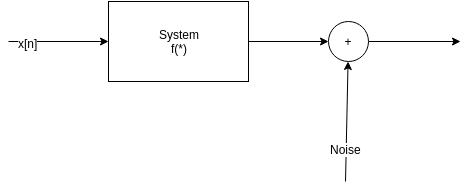
\includegraphics[width=0.8\textwidth]{noisy-system}
	\caption{System with Noisy Output}
	\label{fig:noisy-system}
\end{figure}

\begin{itemize}
	\item Consider noisy system in figure \ref{fig:noisy-system}
	\item For this system $y=\theta^Tx+\eta$ 
	\item Question: is this system LTI?
	\item Answer: $\theta$ must be unbiased to be LTI
   \item How to estimate $\theta$?
	\item Loss functions! Minimize the loss to get the best fit.
\end{itemize}

\section{Loss Functions}%
\begin{itemize}
	 \item Least Squares Loss
	 \item Minimize squares of residuals
	 \item Because of noise, measurement always changes. This means estimator for $\theta$ is also random, because $\hat{\theta}$ depends on $y$ and $y$ depends on noise $\eta$ 
	 \item Bias-Variance Decomposition: expanding MSE definition shows that $MSE[x]=Var[x]+Bias[x]^2$
	 \item Result: biased estimator can have better MSE than unbiased estimator
	 \item norm of biased estimator always better than norm of unbiased estimator
	 \item Ridge regression: squared loss from MSE, + squared norm of $\theta$
	 \item $\lambda$: regularizing term in ridge regression
	 \item Given enough points, it is possible to find an optimal $\lambda$ that is provably best
	 \item Fun stuff: using Bayes theorem, plugging in normal dist for likelihood gets LS estimator, plugging in normal dist for prior leads to ridge regression.
	 \item Review: ML vs MAP estimation
\end{itemize}

\section{Definitions}%
\label{sec:definitions}
\begin{itemize}
	 \item Bias: $Bias[\hat{\theta}] = E[\hat{\theta}]-\theta$ 
	 \item Variance: $Var[\hat{\theta} = E[(\hat{\theta} - E[\hat{\theta}])^2]$
	 \item MSE: $MSE[\hat{\theta}] = E[(\hat{\theta}-\theta)^2]$
\end{itemize}


\end{document}
